% generated by gen_lat_fig.py -- do not edit by hand
\documentclass[10pt]{standalone}
\usepackage{helvet}
\renewcommand{\familydefault}{\sfdefault}
\usepackage{amsmath,amssymb}
\usepackage{tikz}
\usetikzlibrary{arrows.meta,patterns}
\definecolor{wA}{HTML}{9FC5E8}
\definecolor{wB}{HTML}{F6B26B}
\definecolor{wC}{HTML}{93C47D}
\definecolor{wD}{HTML}{C27BA0}
\definecolor{bar}{HTML}{2A78D6}
\newcommand{\fs}{\fontsize{6.4}{7.4}\selectfont}
\newcommand{\fss}{\fontsize{5.8}{6.6}\selectfont}
\begin{document}
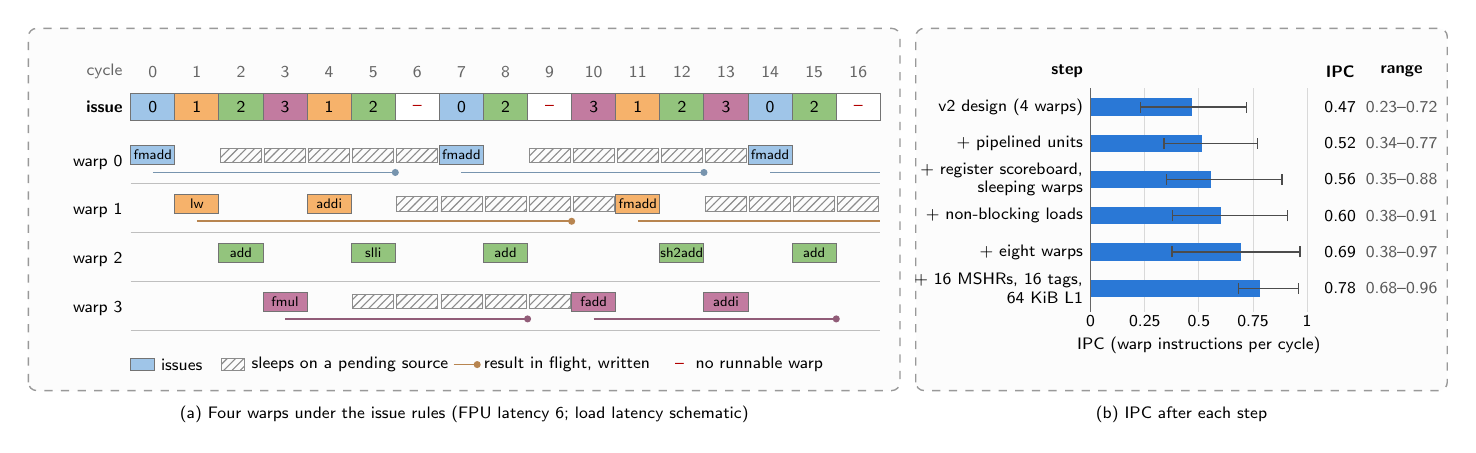
\begin{tikzpicture}[x=1cm, y=1cm,
  tbl/.style={draw=black!55, line width=0.35pt},
  panel/.style={draw=black!40, dashed, rounded corners=3pt, fill=black!1, line width=0.5pt},
  lbl/.style={font=\fs, inner sep=0.5pt},
  cell/.style={font=\fss, inner sep=0.3pt},
  note/.style={font=\fss, inner sep=0.5pt, align=left},
  subcap/.style={font=\fs, inner sep=1pt},
  sleep/.style={draw=black!45, pattern=north east lines, pattern color=black!45, line width=0.3pt},
  arr/.style={-{Latex[length=1.3mm, width=0.9mm]}, line width=0.5pt}]

\draw[panel] (-0.100,-0.050) rectangle (10.970,4.550);
\node[cell, text=black!60] at (1.480,4.000) {0};
\node[cell, text=black!60] at (2.040,4.000) {1};
\node[cell, text=black!60] at (2.600,4.000) {2};
\node[cell, text=black!60] at (3.160,4.000) {3};
\node[cell, text=black!60] at (3.720,4.000) {4};
\node[cell, text=black!60] at (4.280,4.000) {5};
\node[cell, text=black!60] at (4.840,4.000) {6};
\node[cell, text=black!60] at (5.400,4.000) {7};
\node[cell, text=black!60] at (5.960,4.000) {8};
\node[cell, text=black!60] at (6.520,4.000) {9};
\node[cell, text=black!60] at (7.080,4.000) {10};
\node[cell, text=black!60] at (7.640,4.000) {11};
\node[cell, text=black!60] at (8.200,4.000) {12};
\node[cell, text=black!60] at (8.760,4.000) {13};
\node[cell, text=black!60] at (9.320,4.000) {14};
\node[cell, text=black!60] at (9.880,4.000) {15};
\node[cell, text=black!60] at (10.440,4.000) {16};
\node[note, anchor=east, text=black!60] at (1.120,4.000) {cycle};
\node[lbl, anchor=east] at (1.120,3.550) {\textbf{issue}};
\draw[tbl, fill=wA] (1.200,3.380) rectangle (1.760,3.720);
\node[cell] at (1.480,3.550) {0};
\draw[tbl, fill=wB] (1.760,3.380) rectangle (2.320,3.720);
\node[cell] at (2.040,3.550) {1};
\draw[tbl, fill=wC] (2.320,3.380) rectangle (2.880,3.720);
\node[cell] at (2.600,3.550) {2};
\draw[tbl, fill=wD] (2.880,3.380) rectangle (3.440,3.720);
\node[cell] at (3.160,3.550) {3};
\draw[tbl, fill=wB] (3.440,3.380) rectangle (4.000,3.720);
\node[cell] at (3.720,3.550) {1};
\draw[tbl, fill=wC] (4.000,3.380) rectangle (4.560,3.720);
\node[cell] at (4.280,3.550) {2};
\draw[tbl, fill=white] (4.560,3.380) rectangle (5.120,3.720);
\node[cell, text=red!70!black] at (4.840,3.550) {--};
\draw[tbl, fill=wA] (5.120,3.380) rectangle (5.680,3.720);
\node[cell] at (5.400,3.550) {0};
\draw[tbl, fill=wC] (5.680,3.380) rectangle (6.240,3.720);
\node[cell] at (5.960,3.550) {2};
\draw[tbl, fill=white] (6.240,3.380) rectangle (6.800,3.720);
\node[cell, text=red!70!black] at (6.520,3.550) {--};
\draw[tbl, fill=wD] (6.800,3.380) rectangle (7.360,3.720);
\node[cell] at (7.080,3.550) {3};
\draw[tbl, fill=wB] (7.360,3.380) rectangle (7.920,3.720);
\node[cell] at (7.640,3.550) {1};
\draw[tbl, fill=wC] (7.920,3.380) rectangle (8.480,3.720);
\node[cell] at (8.200,3.550) {2};
\draw[tbl, fill=wD] (8.480,3.380) rectangle (9.040,3.720);
\node[cell] at (8.760,3.550) {3};
\draw[tbl, fill=wA] (9.040,3.380) rectangle (9.600,3.720);
\node[cell] at (9.320,3.550) {0};
\draw[tbl, fill=wC] (9.600,3.380) rectangle (10.160,3.720);
\node[cell] at (9.880,3.550) {2};
\draw[tbl, fill=white] (10.160,3.380) rectangle (10.720,3.720);
\node[cell, text=red!70!black] at (10.440,3.550) {--};
\node[lbl, anchor=east] at (1.120,2.850) {warp 0};
\draw[black!25, line width=0.3pt] (1.200,2.580) -- (10.720,2.580);
\draw[tbl, fill=wA] (1.200,2.820) rectangle (1.760,3.060);
\node[cell] at (1.480,2.940) {\fontsize{4.9}{5.4}\selectfont fmadd};
\draw[sleep] (2.340,2.850) rectangle (2.860,3.030);
\draw[sleep] (2.900,2.850) rectangle (3.420,3.030);
\draw[sleep] (3.460,2.850) rectangle (3.980,3.030);
\draw[sleep] (4.020,2.850) rectangle (4.540,3.030);
\draw[sleep] (4.580,2.850) rectangle (5.100,3.030);
\draw[tbl, fill=wA] (5.120,2.820) rectangle (5.680,3.060);
\node[cell] at (5.400,2.940) {\fontsize{4.9}{5.4}\selectfont fmadd};
\draw[sleep] (6.260,2.850) rectangle (6.780,3.030);
\draw[sleep] (6.820,2.850) rectangle (7.340,3.030);
\draw[sleep] (7.380,2.850) rectangle (7.900,3.030);
\draw[sleep] (7.940,2.850) rectangle (8.460,3.030);
\draw[sleep] (8.500,2.850) rectangle (9.020,3.030);
\draw[tbl, fill=wA] (9.040,2.820) rectangle (9.600,3.060);
\node[cell] at (9.320,2.940) {\fontsize{4.9}{5.4}\selectfont fmadd};
\draw[line width=0.6pt, draw=wA!75!black] (1.480,2.720) -- (4.560,2.720);
\fill[wA!75!black] (4.560,2.720) circle (0.045);
\draw[line width=0.6pt, draw=wA!75!black] (5.400,2.720) -- (8.480,2.720);
\fill[wA!75!black] (8.480,2.720) circle (0.045);
\draw[line width=0.6pt, draw=wA!75!black] (9.320,2.720) -- (10.720,2.720);
\node[lbl, anchor=east] at (1.120,2.230) {warp 1};
\draw[black!25, line width=0.3pt] (1.200,1.960) -- (10.720,1.960);
\draw[tbl, fill=wB] (1.760,2.200) rectangle (2.320,2.440);
\node[cell] at (2.040,2.320) {\fontsize{4.9}{5.4}\selectfont lw};
\draw[tbl, fill=wB] (3.440,2.200) rectangle (4.000,2.440);
\node[cell] at (3.720,2.320) {\fontsize{4.9}{5.4}\selectfont addi};
\draw[sleep] (4.580,2.230) rectangle (5.100,2.410);
\draw[sleep] (5.140,2.230) rectangle (5.660,2.410);
\draw[sleep] (5.700,2.230) rectangle (6.220,2.410);
\draw[sleep] (6.260,2.230) rectangle (6.780,2.410);
\draw[sleep] (6.820,2.230) rectangle (7.340,2.410);
\draw[tbl, fill=wB] (7.360,2.200) rectangle (7.920,2.440);
\node[cell] at (7.640,2.320) {\fontsize{4.9}{5.4}\selectfont fmadd};
\draw[sleep] (8.500,2.230) rectangle (9.020,2.410);
\draw[sleep] (9.060,2.230) rectangle (9.580,2.410);
\draw[sleep] (9.620,2.230) rectangle (10.140,2.410);
\draw[sleep] (10.180,2.230) rectangle (10.700,2.410);
\draw[line width=0.6pt, draw=wB!75!black] (2.040,2.100) -- (6.800,2.100);
\fill[wB!75!black] (6.800,2.100) circle (0.045);
\draw[line width=0.6pt, draw=wB!75!black] (7.640,2.100) -- (10.720,2.100);
\node[lbl, anchor=east] at (1.120,1.610) {warp 2};
\draw[black!25, line width=0.3pt] (1.200,1.340) -- (10.720,1.340);
\draw[tbl, fill=wC] (2.320,1.580) rectangle (2.880,1.820);
\node[cell] at (2.600,1.700) {\fontsize{4.9}{5.4}\selectfont add};
\draw[tbl, fill=wC] (4.000,1.580) rectangle (4.560,1.820);
\node[cell] at (4.280,1.700) {\fontsize{4.9}{5.4}\selectfont slli};
\draw[tbl, fill=wC] (5.680,1.580) rectangle (6.240,1.820);
\node[cell] at (5.960,1.700) {\fontsize{4.9}{5.4}\selectfont add};
\draw[tbl, fill=wC] (7.920,1.580) rectangle (8.480,1.820);
\node[cell] at (8.200,1.700) {\fontsize{4.9}{5.4}\selectfont sh2add};
\draw[tbl, fill=wC] (9.600,1.580) rectangle (10.160,1.820);
\node[cell] at (9.880,1.700) {\fontsize{4.9}{5.4}\selectfont add};
\node[lbl, anchor=east] at (1.120,0.990) {warp 3};
\draw[black!25, line width=0.3pt] (1.200,0.720) -- (10.720,0.720);
\draw[tbl, fill=wD] (2.880,0.960) rectangle (3.440,1.200);
\node[cell] at (3.160,1.080) {\fontsize{4.9}{5.4}\selectfont fmul};
\draw[sleep] (4.020,0.990) rectangle (4.540,1.170);
\draw[sleep] (4.580,0.990) rectangle (5.100,1.170);
\draw[sleep] (5.140,0.990) rectangle (5.660,1.170);
\draw[sleep] (5.700,0.990) rectangle (6.220,1.170);
\draw[sleep] (6.260,0.990) rectangle (6.780,1.170);
\draw[tbl, fill=wD] (6.800,0.960) rectangle (7.360,1.200);
\node[cell] at (7.080,1.080) {\fontsize{4.9}{5.4}\selectfont fadd};
\draw[tbl, fill=wD] (8.480,0.960) rectangle (9.040,1.200);
\node[cell] at (8.760,1.080) {\fontsize{4.9}{5.4}\selectfont addi};
\draw[line width=0.6pt, draw=wD!75!black] (3.160,0.860) -- (6.240,0.860);
\fill[wD!75!black] (6.240,0.860) circle (0.045);
\draw[line width=0.6pt, draw=wD!75!black] (7.080,0.860) -- (10.160,0.860);
\fill[wD!75!black] (10.160,0.860) circle (0.045);
\draw[tbl, fill=wA] (1.200,0.200) rectangle (1.500,0.360);
\node[note, anchor=west] at (1.560,0.280) {issues};
\draw[sleep] (2.350,0.200) rectangle (2.650,0.360);
\node[note, anchor=west] at (2.710,0.280) {sleeps on a pending source};
\draw[line width=0.6pt, draw=wB!75!black] (5.300,0.280) -- (5.600,0.280);
\fill[wB!75!black] (5.600,0.280) circle (0.045);
\node[note, anchor=west] at (5.660,0.280) {result in flight, written};
\node[cell, text=red!70!black] at (8.170,0.280) {--};
\node[note, anchor=west] at (8.350,0.280) {no runnable warp};
\node[subcap] at (5.435,-0.350) {(a) Four warps under the issue rules (FPU latency 6; load latency schematic)};
\draw[panel] (11.170,-0.050) rectangle (17.920,4.550);
\node[cell, anchor=east] at (13.310,4.000) {\textbf{step}};
\node[cell] at (16.560,4.000) {\textbf{IPC}};
\node[cell] at (17.340,4.000) {\textbf{range}};
\draw[black!15, line width=0.3pt] (13.390,0.950) -- (13.390,3.790);
\node[cell, anchor=north] at (13.390,0.920) {0};
\draw[black!15, line width=0.3pt] (14.078,0.950) -- (14.078,3.790);
\node[cell, anchor=north] at (14.078,0.920) {0.25};
\draw[black!15, line width=0.3pt] (14.765,0.950) -- (14.765,3.790);
\node[cell, anchor=north] at (14.765,0.920) {0.5};
\draw[black!15, line width=0.3pt] (15.453,0.950) -- (15.453,3.790);
\node[cell, anchor=north] at (15.453,0.920) {0.75};
\draw[black!15, line width=0.3pt] (16.140,0.950) -- (16.140,3.790);
\node[cell, anchor=north] at (16.140,0.920) {1};
\draw[black!60, line width=0.45pt] (13.390,0.950) -- (13.390,3.790);
\node[cell, anchor=north] at (14.765,0.650) {IPC (warp instructions per cycle)};
\node[cell, anchor=east, align=right] at (13.310,3.550) {v2 design (4 warps)};
\fill[bar] (13.390,3.440) rectangle (14.672,3.660);
\draw[black!70, line width=0.45pt] (14.028,3.550) -- (15.368,3.550);
\draw[black!70, line width=0.45pt] (14.028,3.480) -- (14.028,3.620);
\draw[black!70, line width=0.45pt] (15.368,3.480) -- (15.368,3.620);
\node[cell] at (16.560,3.550) {0.47};
\node[cell, text=black!65] at (17.340,3.550) {0.23--0.72};
\node[cell, anchor=east, align=right] at (13.310,3.090) {+ pipelined units};
\fill[bar] (13.390,2.980) rectangle (14.808,3.200);
\draw[black!70, line width=0.45pt] (14.321,3.090) -- (15.512,3.090);
\draw[black!70, line width=0.45pt] (14.321,3.020) -- (14.321,3.160);
\draw[black!70, line width=0.45pt] (15.512,3.020) -- (15.512,3.160);
\node[cell] at (16.560,3.090) {0.52};
\node[cell, text=black!65] at (17.340,3.090) {0.34--0.77};
\node[cell, anchor=east, align=right] at (13.310,2.630) {+ register scoreboard,\\sleeping warps};
\fill[bar] (13.390,2.520) rectangle (14.917,2.740);
\draw[black!70, line width=0.45pt] (14.352,2.630) -- (15.822,2.630);
\draw[black!70, line width=0.45pt] (14.352,2.560) -- (14.352,2.700);
\draw[black!70, line width=0.45pt] (15.822,2.560) -- (15.822,2.700);
\node[cell] at (16.560,2.630) {0.56};
\node[cell, text=black!65] at (17.340,2.630) {0.35--0.88};
\node[cell, anchor=east, align=right] at (13.310,2.170) {+ non-blocking loads};
\fill[bar] (13.390,2.060) rectangle (15.043,2.280);
\draw[black!70, line width=0.45pt] (14.433,2.170) -- (15.891,2.170);
\draw[black!70, line width=0.45pt] (14.433,2.100) -- (14.433,2.240);
\draw[black!70, line width=0.45pt] (15.891,2.100) -- (15.891,2.240);
\node[cell] at (16.560,2.170) {0.60};
\node[cell, text=black!65] at (17.340,2.170) {0.38--0.91};
\node[cell, anchor=east, align=right] at (13.310,1.710) {+ eight warps};
\fill[bar] (13.390,1.600) rectangle (15.296,1.820);
\draw[black!70, line width=0.45pt] (14.423,1.710) -- (16.048,1.710);
\draw[black!70, line width=0.45pt] (14.423,1.640) -- (14.423,1.780);
\draw[black!70, line width=0.45pt] (16.048,1.640) -- (16.048,1.780);
\node[cell] at (16.560,1.710) {0.69};
\node[cell, text=black!65] at (17.340,1.710) {0.38--0.97};
\node[cell, anchor=east, align=right] at (13.310,1.250) {+ 16 MSHRs, 16 tags,\\64 KiB L1};
\fill[bar] (13.390,1.140) rectangle (15.547,1.360);
\draw[black!70, line width=0.45pt] (15.264,1.250) -- (16.030,1.250);
\draw[black!70, line width=0.45pt] (15.264,1.180) -- (15.264,1.320);
\draw[black!70, line width=0.45pt] (16.030,1.180) -- (16.030,1.320);
\node[cell] at (16.560,1.250) {0.78};
\node[cell, text=black!65] at (17.340,1.250) {0.68--0.96};
\node[subcap] at (14.545,-0.350) {(b) IPC after each step};
\end{tikzpicture}
\end{document}
